%**************************************************************************************
% License:
% CC BY-NC-SA 4.0 (http://creativecommons.org/licenses/by-nc-sa/4.0/)
%**************************************************************************************

\documentclass[notes]{beamer}

\mode<presentation> {

\usetheme{Madrid}

% Burnt orange
\definecolor{burntorange}{rgb}{0.8, 0.33, 0.0}
\colorlet{beamer@blendedblue}{burntorange}
% Pale yellow
\definecolor{paleyellow}{rgb}{1.0, 1.0, 0.953}
\setbeamercolor{background canvas}{bg=paleyellow}
% Secondary and tertiary palett
\setbeamercolor*{palette secondary}{use=structure,fg=white,bg=burntorange!80!black}
\setbeamercolor*{palette tertiary}{use=structure,fg=white,bg=burntorange!60!black}

% To remove the footer line in all slides uncomment this line
%\setbeamertemplate{footline}
% To replace the footer line in all slides with a simple slide count uncomment this line
%\setbeamertemplate{footline}[page number]

% To remove the navigation symbols from the bottom of all slides uncomment this line
%\setbeamertemplate{navigation symbols}{}
}

\usepackage{amsmath}
\usepackage{bm}
\usepackage{booktabs} % Allows the use of \toprule, \midrule and \bottomrule in tables
\usepackage{breqn}
\usepackage{cleveref}
\usepackage{graphicx} % for figures
\usepackage[labelsep=space,tableposition=top]{caption}
\renewcommand{\figurename}{Fig.} 
\usepackage{caption,subcaption}% http://ctan.org/pkg/{caption,subcaption}
\usepackage{xcolor}


% To print 2 slides on a page
%\usepackage{handoutWithNotes}
%\pgfpagesuselayout{2 on 1}[border shrink=2mm]

%----------------------------------------------------------------------------------------
%	TITLE PAGE
%----------------------------------------------------------------------------------------
% The short title appears at the bottom of every slide, the full title is only on the title page
\title[CE394M: 1D - FEM]{CE394M: 1D-Finite Element Method} 
\author{Krishna Kumar} % name
\institute[UT Austin] % institution 
{
University of Texas at Austin \\
\medskip
\textit{
  \url{krishnak@utexas.edu}} % Your email address
}
\date{\today} % Date, can be changed to a custom date

\begin{document}

\begin{frame}
\titlepage % title page as the first slide
\end{frame}

\begin{frame}
 % Table of contents slide, comment this block out to remove it
 \frametitle{Overview}
 % Throughout your presentation, if you choose to use \section{} and \subsection{} 
 % commands, these %will automatically be printed on this slide as an overview 
 \tableofcontents
\end{frame}

%----------------------------------------------------------------------------------------
% slides
%----------------------------------------------------------------------------------------
\section{FEM workflow}
%------------------------------------------------
\begin{frame}
\frametitle{Finite Element Analysis}
\begin{figure}[ht]
	\centering
	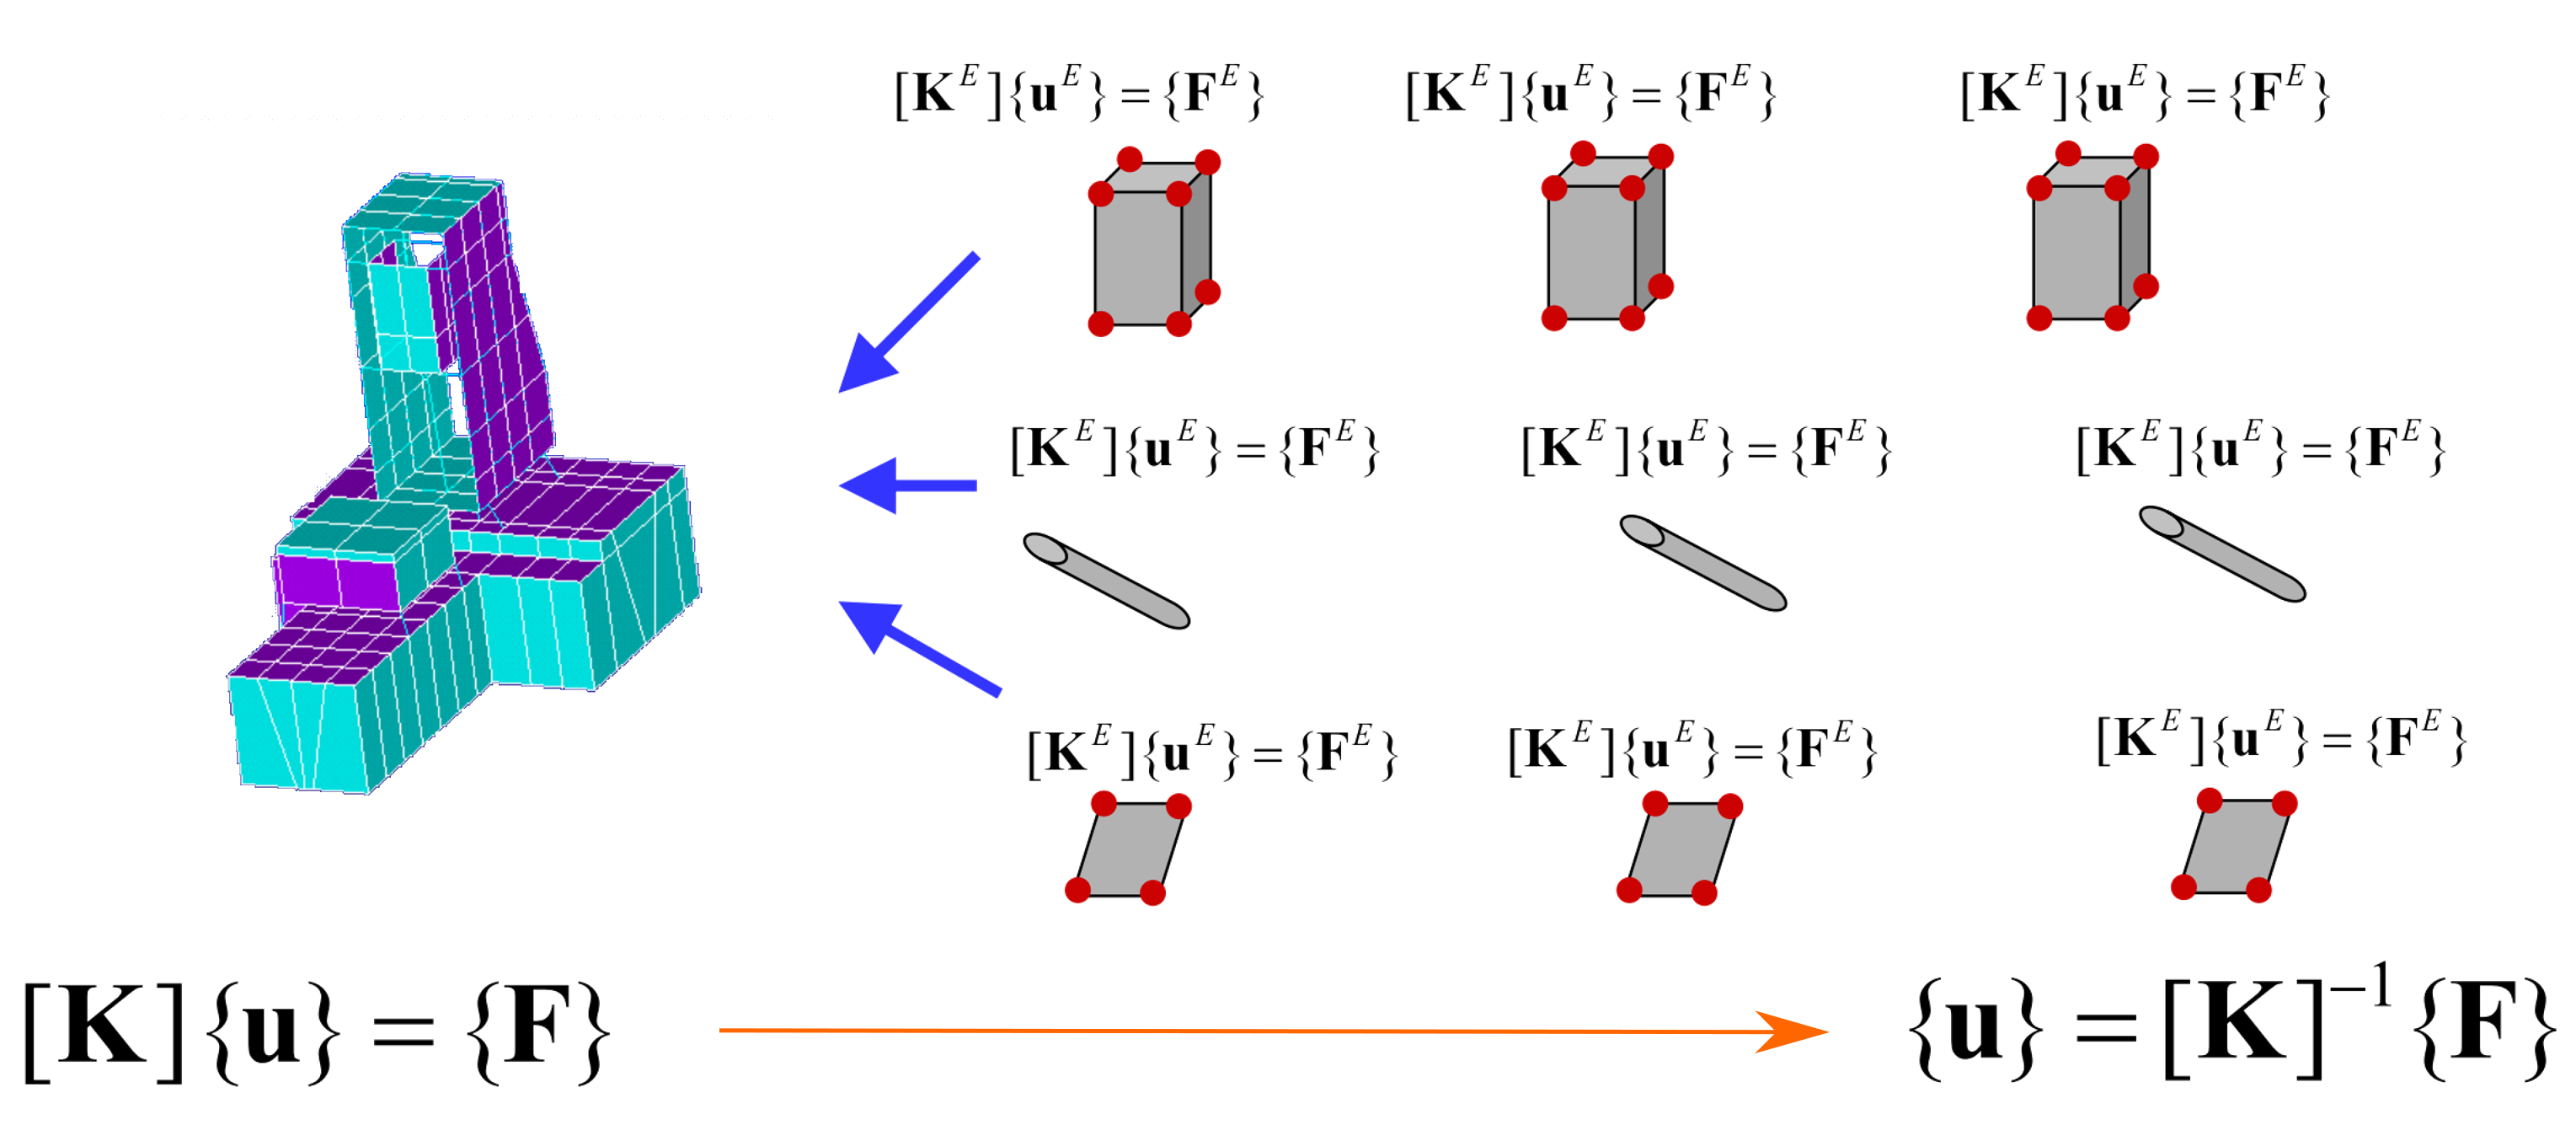
\includegraphics[width=\textwidth]{figs/fem.png}
\end{figure}
\end{frame}

%------------------------------------------------
\begin{frame}
\frametitle{Finite Element Analysis}
FEM is a systematic procedure for approximating differential equations. For any problem in any spatial dimension it follows the same steps:
\mode<beamer>{
\begin{enumerate}
\item Identify the equation of interest
\item Cast the equation of interest in a weak form
\item Select a finite element type
\item Construct the element matrix and vector
\item Assemble the global matrix and vector and apply boundary conditions
\item Solve the system of linear equations
\end{enumerate}
}
\mode<handout>{
\vspace{5cm}
}
\end{frame}

%---------------------------------------------------
\section{1D FEM}
%------------------------------------------------
\begin{frame}
\frametitle{1D Finite Element Analysis of a cantilever beam}
\begin{figure}[ht]
	\centering
	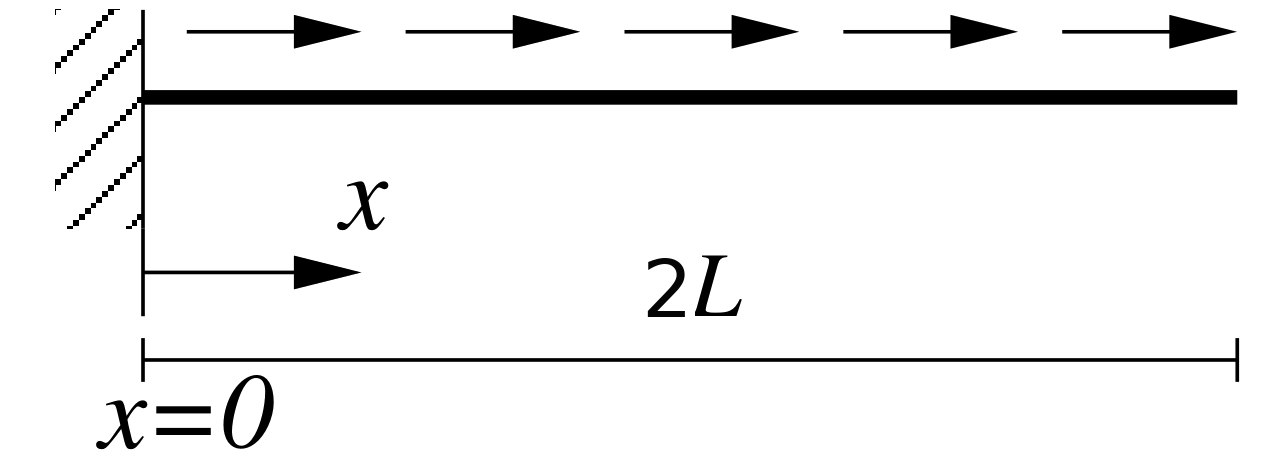
\includegraphics[width=\textwidth]{figs/cantilever.png}
	\caption*{1D cantilever beam}
\end{figure}
Assume $L$ as unit length $L = 1$. Unit force $f = 1$.
\end{frame}

%------------------------------------------------
\begin{frame}
\frametitle{1D Finite Element Analysis of a cantilever beam}
What element should be used?
\begin{figure}[ht]
	\centering
	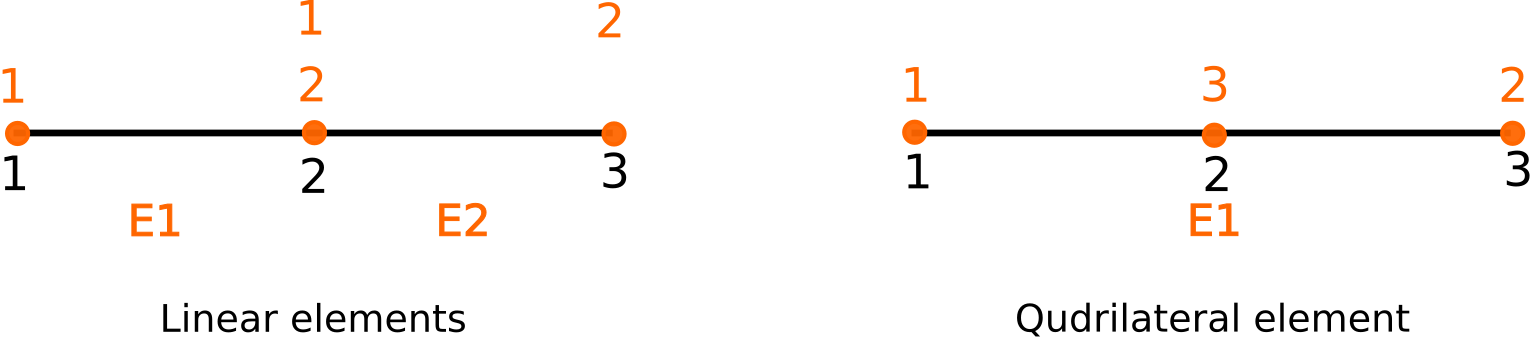
\includegraphics[width=\textwidth]{figs/fem-cantilever-linear-quad.png}
	\caption*{1D discretization of a cantilever beam}
\end{figure}
\end{frame}

%------------------------------------------------
\begin{frame}
\frametitle{1D FEM: Shape functions and derivatives}
Shape function $\mathbf{N}$:
\mode<beamer>{
	\begin{equation*}
		\mathbf{N} = \left[
			1-\frac{x}{L} \qquad
			 \frac{x}{L} 
		\right]
	\end{equation*}
	\begin{equation*}
		\mathbf{N} = \left[
			1-x \qquad
			x \right]
	\end{equation*}
}
\mode<handout>{
	\vspace{2.5cm}
}
$\mathbf{B}$ is the derivatives of the shape functions:
\mode<beamer>{
	\begin{equation*}
		\mathbf{B} = \left[\frac{dN_1(x)}{dx} \qquad \frac{dN_2(x)}{dx}\right]
	\end{equation*}
	
	\begin{equation*}
		\mathbf{B} = \left[\frac{-1}{L} \qquad \frac{1}{L}\right]  = \left[-1 \quad 1\right]
	\end{equation*}
}
\mode<handout>{
	\vspace{2.5cm}
}
In matrix format: \mode<beamer>{$ u_h = \mathbf{Na_e} $ and $\epsilon_h = \mathbf{Ba_e}$.}
\end{frame}


%------------------------------------------------
\begin{frame}
\frametitle{1D FEM: Stiffness and force}
Element stiffness $k_e$:
\mode<beamer>{
	\begin{equation*}
		k_e = \int \mathbf{B}^T EA \, \mathbf{B}\, \mathrm{d}x = \int_0^L
		\left[ \begin{matrix} \frac{dN_1}{dx} \\ \frac{dN_2}{dx} \end{matrix} \right] EA
		\left[ \begin{matrix} \frac{dN_1}{dx} & \frac{dN_2}{dx}  \end{matrix} \right] dx
	\end{equation*}
	
	\begin{equation*}
		k_e = EA
		\begin{bmatrix}
		 1 & -1 \\
		-1 &  1 \\
		\end{bmatrix}
	\end{equation*}
}
\mode<handout>{
	\vspace{2.5cm}
}
Right-hand side vector $b_e$ is:
\mode<beamer>{
	\begin{equation*}
	b_e = \int \mathbf{N}^T \, f\, \mathrm{d}x = \int_0^L 	\begin{bmatrix}
	-\frac{x}{L} + 1\\
	\frac{x}{L}\\
	\end{bmatrix}  =  \begin{bmatrix}
	-\frac{x^2}{2L} + x\\
	\frac{x^2}{2L}\\
	\end{bmatrix}_0^L%
	 =  \begin{bmatrix}
	-\frac{x^2}{2} + x\\
	\frac{x^2}{2}\\
	\end{bmatrix}_0^1
	\end{equation*}
	
	\begin{equation*}
		b_e =
		\begin{bmatrix}
			\frac{1}{2}\\
			\frac{1}{2}\\
		\end{bmatrix}
	\end{equation*}
}
\mode<handout>{
	\vspace{2.5cm}
}
\end{frame}

\note{
	The force vector $b_e$ should be equal to the total sum of all the forces acting on the element. 
	Here we have a unit force over a unit length so the total force is $1 \cdot 1 = 1$. This force of 1 is
	distributed over the two nodes as $\begin{bmatrix}\frac{1}{2} \\ \frac{1}{2} \\\end{bmatrix}$.
}

%-------------------------------------------------
\section{Assembly}

%------------------------------------------------
\begin{frame}
\frametitle{1D FEM: Assembly}
\begin{figure}[ht]
	\centering
	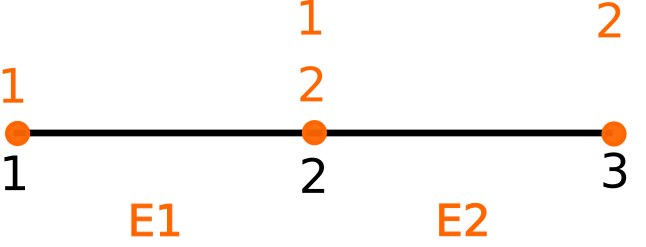
\includegraphics[width=0.5\textwidth]{figs/fem-cantilever-linear.png}
\end{figure}
Element stiffness $k_e$:
\begin{align*}
	k_e & = %
		\begin{bmatrix}
			k_{11} & k_{12} \\
			k_{21} & k_{22} \\
		\end{bmatrix} \\
		%
		\\
	 & = EA %
		\begin{bmatrix}
			1 & -1 \\
			-1 &  1 \\
		\end{bmatrix}
\end{align*}
\mode<beamer>{
}
\mode<handout>{
	\vspace{4cm}
}
\end{frame}

\note{
	To perform a FE analysis, the element matrices and vectors are computed for each element and inserted into the global stiffness matrix \textbf{K} and global right-hand side vector \textbf{b}. The system $\mathrm{Ka} = \mathrm{b}$ is then solved to yield $\textbf{a}$. The process of inserting the element matrices and vectors into their global counterparts is known as assembly. A local (element) degree of freedom corresponds to a global degree of freedom, and an entry in a local matrix or vector is copied to its corresponding position in the global matrix.
}


%------------------------------------------------
\begin{frame}
\frametitle{1D FEM: Assembly}
\begin{figure}[ht]
	\centering
	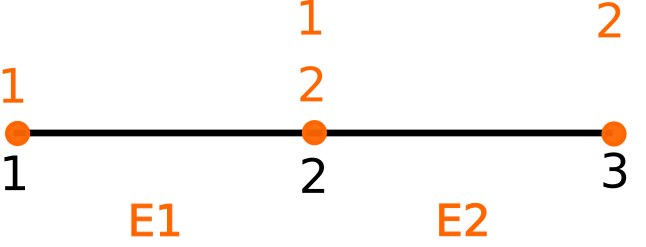
\includegraphics[width=0.5\textwidth]{figs/fem-cantilever-linear.png}
\end{figure}
\mode<beamer>{
	\begin{table}
		\begin{tabular}{lcccc}
			\toprule
			& \multicolumn{2}{c}{\textbf{element 1}} & \multicolumn{2}{c}{\textbf{element 2}} \\
			\midrule
			Local dof  & 1	& 2 & 1 & 2 \\
			Global dof & 1  & 2	& 2 & 3 \\          
			\bottomrule
		\end{tabular}
	\end{table}
}
\mode<handout>{
	\begin{table}
		\begin{tabular}{lcccc}
			\toprule
			& \multicolumn{2}{c}{\textbf{element 1}} & \multicolumn{2}{c}{\textbf{element 2}} \\
			\midrule
			Local dof  &  &	 &  &\\
			Global dof &  &	 &  &\\     
			\bottomrule
		\end{tabular}
	\end{table}
	\vspace{1cm}
}
\end{frame}


%------------------------------------------------
\begin{frame}
\frametitle{1D FEM: Global stiffness matrix}
\begin{figure}[ht]
	\centering
	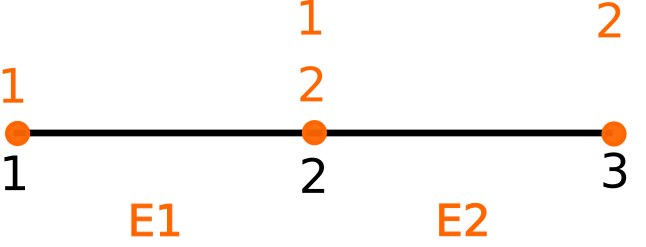
\includegraphics[width=0.4\textwidth]{figs/fem-cantilever-linear.png}
\end{figure}
Global stiffness \textbf{K}:

\mode<beamer>{
	\begin{align*}
	k_e & = %
	\begin{bmatrix}
	k_{11}^1 & k_{12}^1 & \textcolor{red}{0} \\
	k_{21}^1 & k_{22}^1 + \textcolor{blue}{k_{11}^2} & \textcolor{blue}{k_{12}^2} \\
	\textcolor{red}{0}  & \textcolor{blue}{k_{21}^2} & \textcolor{blue}{k_{22}^2} \\ 
	\end{bmatrix} \\
	%
	\\
	& = EA %
	\begin{bmatrix}
	1 & -1 & 0\\
	-1 &  1 + \textcolor{blue}{1} & \textcolor{blue}{-1}\\
	0 & \textcolor{blue}{-1} & \textcolor{blue}{1} \\
	\end{bmatrix} = EA%
	\begin{bmatrix}
	1 & -1 & 0\\
	-1 &  2 & -1\\
	0 & -1 & 1 \\
	\end{bmatrix}
	\end{align*}
Where superscripts in $k_{ij}^e$ denotes element numbering.
}
\mode<handout>{
	\vspace{5cm}
}
\end{frame}

%------------------------------------------------
\begin{frame}
\frametitle{Boundary conditions}
\begin{figure}[ht]
	\centering
	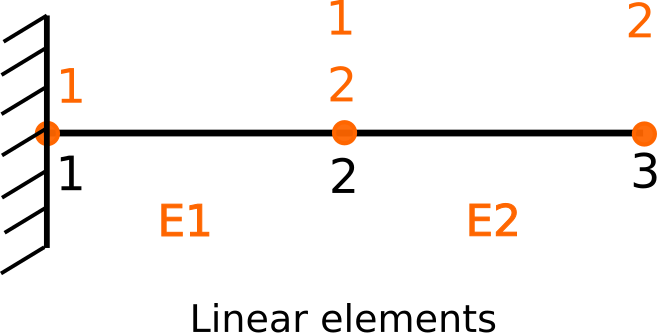
\includegraphics[width=0.4\textwidth]{figs/fem-cantilever-linear-bc.png}
\end{figure}
Global stiffness \textbf{K}:

\mode<beamer>{
	\begin{align*}
	\textbf{K} & = %
	\begin{bmatrix}
	k_{11}^1 & k_{12}^1 & \textcolor{red}{0} \\
	k_{21}^1 & k_{22}^1 + \textcolor{blue}{k_{11}^2} & \textcolor{blue}{k_{12}^2} \\
	\textcolor{red}{0}  & \textcolor{blue}{k_{21}^2} & \textcolor{blue}{k_{22}^2} \\ 
	\end{bmatrix} \\
	%
	\\
	& = EA %
	\begin{bmatrix}
	1 & -1 & 0\\
	-1 &  1 + \textcolor{blue}{1} & \textcolor{blue}{-1}\\
	0 & \textcolor{blue}{-1} & \textcolor{blue}{1} \\
	\end{bmatrix} = EA%
	\begin{bmatrix}
	1 & -1 & 0\\
	-1 &  2 & -1\\
	0 & -1 & 1 \\
	\end{bmatrix}
	\end{align*}
	Where superscripts in $k_{ij}^e$ denotes element numbering.
}
\mode<handout>{
	\vspace{5cm}
}
\end{frame}

\note{
	\textit{\textbf{Neumann (force) boundary conditions }}appear naturally in the weak form 
	of the equilibrium equation, and therefore do not require special consideration. 
	In the context of variational methods, they are sometimes referred to as 
	`\textit{natural boundary conditions}'. \\
	
	However, \textbf{\textit{Dirichlet (displacement) boundary conditions}} still need to be applied. If we fail to apply proper displacement boundary 
	conditions, the stiffness matrix will be singular, meaning that there is no unique solution. 
	In the context of variational methods, displacement boundary conditions are often referred to as `\textit{essential boundary conditions}'.}

\note{
	There are two approaches that are commonly used to apply displacement boundary
	conditions. One is to modify terms in the global stiffness matrix and place the displacement 
	boundary condition in the right-hand side vector, and the other is to eliminate the
	degrees of freedom associated with a displacement boundary condition from the global
	system of equations.
}


%------------------------------------------------
\begin{frame}
\frametitle{Applying boundary conditions: Approach I}
Consider a global system that has already been assembled by adding the contribution of
each element:
\begin{equation*}
	\begin{bmatrix}
		K_{11} & K_{12} & 0 & 0 & 0 \\
		K_{21} & K_{22} & K_{23} & 0 & 0 \\
		0 & K_{32} & K_{33} & K_{34} & 0 \\
		0 & 0 & K_{43} & K_{44} & K_{45} \\
		0 & 0 & 0  &  K_{54} & K_{55}\\
	\end{bmatrix} %
	\begin{bmatrix}
		a_1 \\
		a_2 \\
		a_3 \\
		a_4 \\
		a_5 \\
	\end{bmatrix} =  %
	\begin{bmatrix}
		b_1 \\
		b_2 \\
		b_3 \\
		b_4 \\
		b_5 \\
	\end{bmatrix}
\end{equation*}
To apply a displacement of $g$ at node one ($a_1 = g$):

\mode<beamer>{
we can zero the first row of the matrix, place a `one' on the diagonal and set $b_1 = g$,
	\begin{equation*}
	\begin{bmatrix}
		\textcolor{red}{1} & \textcolor{red}{0} & \textcolor{red}{0} & \textcolor{red}{0} & \textcolor{red}{0} \\
		K_{21} & K_{22} & K_{23} & 0 & 0 \\
		0 & K_{32} & K_{33} & K_{34} & 0 \\
		0 & 0 & K_{43} & K_{44} & K_{45} \\
		0 & 0 & 0  &  K_{54} & K_{55} \\
	\end{bmatrix} %
	\begin{bmatrix}
		\textcolor{red}{a_1} \\
		a_2 \\
		a_3 \\
		a_4 \\
		a_5 \\
	\end{bmatrix} = %
	\begin{bmatrix}
		\textcolor{red}{g} \\
		b_2 \\
		b_3 \\
		b_4 \\
		b_5 \\
	\end{bmatrix}
	\end{equation*}
}
\mode<handout>{
	\vspace{5cm}
}
\end{frame}

\note{
	Multiplying the top row of the matrix by the vector \textbf{\textit{a}}, we can see that solving this system of equations will lead to $a_1 = g$. There is however a significant drawback to
	this technique: if the matrix was originally symmetric, we have destroyed the symmetry.
	We will not to be able to use any specialised linear solvers that exploit symmetry of a
	matrix, which will possibly double the solution time. For $g = 0$ we could also zero the
	first column and preserve symmetry, but this is not possible for $g \ne 0$.}


%------------------------------------------------
\begin{frame}
\frametitle{Applying boundary conditions: Approach II}
Prescribe the displacement at nodes 1 \& 2, all entries in rows one and two in \textbf{K} and \textbf{b} will be equal to zero:
\mode<beamer>{
\begin{equation*}
\begin{bmatrix}
0 & 0 & 0 & 0 & 0 \\
0 & 0 & 0 & 0 & 0 \\
0 & K_{32} & K_{33} & K_{34} & 0 \\
0 & 0 & K_{43} & K_{44} & K_{45} \\
0 & 0 & 0  &  K_{54} & K_{55}\\
\end{bmatrix} %
\begin{bmatrix}
g_1 \\
g_2 \\
a_3 \\
a_4 \\
a_5 \\
\end{bmatrix} =  %
\begin{bmatrix}
0 \\
0 \\
b_3 \\
b_4 \\
b_5 \\
\end{bmatrix}
\end{equation*}
}
\mode<handout>{
	\vspace{3cm}
}
Since the $g$ terms are known, we can take them to the right-hand side of the equation:
\mode<beamer>{
	\begin{equation*}
	\begin{bmatrix}
		K_{33} & K_{34} & 0 \\
		K_{43} & K_{44} & K_{45} \\
		0  &  K_{54} & K_{55} \\
	\end{bmatrix} %
	\begin{bmatrix}
		a_3 \\
		a_4 \\
		a_5 \\
	\end{bmatrix} =  %
	\begin{bmatrix}
		b_3 \\
		b_4 \\
		b_5 \\
	\end{bmatrix} - %
	\begin{bmatrix}
		0 & K_{32} \\
		0 & 0 \\
		0 & 0 \\
	\end{bmatrix} %
	\begin{bmatrix}
		g_1 \\
		g_2 \\
	\end{bmatrix}  %
	\end{equation*}
}
\mode<handout>{
	\vspace{3cm}
}
\end{frame}

\note{
The second approach is to eliminate the degrees of freedom where the displacement
is prescribed. Firstly, recall that wherever a displacement condition is applied, the weight
function must be equal to zero.

Now we have smaller matrix and any symmetry is preserved. This technique can be
applied element-wise during assembly of the global matrix and it is used by finite element
programs aimed at solid and structural mechanics. It is however more complicated to
program than the first approach.}

%------------------------------------------------
\begin{frame}
\frametitle{Global system of equations}
Assemble the global system of equations:
\begin{equation*}
\mathbf{K} = 
\begin{bmatrix}
	k_{11}^1 & k_{12}^1 & \textcolor{red}{0} \\
	k_{21}^1 & k_{22}^1 + \textcolor{blue}{k_{11}^2} & \textcolor{blue}{k_{12}^2} \\
	\textcolor{red}{0}  & \textcolor{blue}{k_{21}^2} & \textcolor{blue}{k_{22}^2} \\ 
\end{bmatrix}
\begin{bmatrix}
a_1 \\
a_2 \\
a_3 \\
\end{bmatrix} = %
\begin{bmatrix}
b_1 \\
b_2 \\
b_3 \\
\end{bmatrix}
\end{equation*}

\mode<beamer>{
	\begin{equation*}
	\mathbf{K} = 
	\begin{bmatrix}
		1 & -1 &  0  \\
	   -1 &  2 & -1 \\
		0 & -1 &  1 \\ 
	\end{bmatrix}
	\begin{bmatrix}
		0 \\
		a_2 \\
		a_3 \\
	\end{bmatrix} = %
	\begin{bmatrix}
		1/2 \\
		1 \\
		1/2 \\
	\end{bmatrix}
	\end{equation*}
}
\mode<handout>{
	\vspace{3cm}
}
\end{frame}


%------------------------------------------------
\begin{frame}
\frametitle{Applying boundary conditions}
Assemble the global system of equations:
\begin{equation*}
\begin{bmatrix}
1 & -1 &  0  \\
-1 &  2 & -1 \\
0 & -1 &  1 \\ 
\end{bmatrix}
\begin{bmatrix}
0 \\
a_2 \\
a_3 \\
\end{bmatrix} = %
\begin{bmatrix}
1/2 \\
1 \\
1/2 \\
\end{bmatrix}
\end{equation*}
We need to apply the boundary condition $u(0) = 0$, which requires that $a_1 = 0$. The
simplest way to impose this condition is to delete the first row and column of the
stiffness matrix:
\mode<beamer>{
	\begin{equation*}
	\begin{bmatrix}
		2 & -1 \\
	   -1 &  1 \\ 
	\end{bmatrix}
	\begin{bmatrix}
		a_2 \\
		a_3 \\
	\end{bmatrix} = %
	\begin{bmatrix}
		1 \\
		1/2 \\
	\end{bmatrix}
	\end{equation*}
}
\mode<handout>{
	\vspace{2cm}
}
Solving this system we have: \mode<beamer>{$a^T = (1/EA)\left[0 \quad 1.5 \quad 2.0 \right]$.}
\end{frame}

%------------------------------------------------
\begin{frame}
\frametitle{Analytical solution of a 1D cantilever beam}
The Euler–Bernoulli equation describes the relationship between the beam's deflection and the applied load:
\begin{equation*}
	-EA\frac{d^2u}{dx^2} = 1
\end{equation*}
The exact solution is:
\begin{equation*}
	u = \frac{1}{EA}(\frac{-x^2}{2} + Cx + D)
\end{equation*}
Using the boundary conditions: $u(0) = 0$ and $\frac{du(2)}{dx} = 0$. 
\mode<beamer>{
	\begin{equation*}
		u = \frac{1}{EA}(\frac{-x^2}{2} + 2)
	\end{equation*}
}
\mode<handout>{
	\vspace{1.5cm}
}
\end{frame}

\note{
The finite element solution is exact at the nodes, but it is not exact between the nodes. This `\textit{exactness}' is a feature of finite element methods in one dimension, but it does not carry over to higher dimensions.}


\section{Errors in the FEM}
%------------------------------------------------
\begin{frame}
\frametitle{Error in the Finite Element Methods}
This nodal `\textit{exactness}' means that looking at error in the displacement at the nodes does not tell us about the error. Displacement error norm:
\mode<beamer>{
\begin{equation*}
	e_u = \left(\int_0^L (u - u_h)^2 \, \mathrm{d}x \right)
\end{equation*}
\begin{figure}
	\centering
	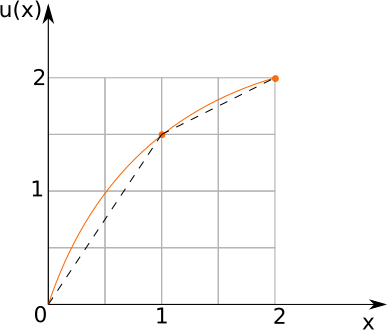
\includegraphics[width=0.5\textwidth]{figs/1d-beam-fem-results.png}
\end{figure}
}
\mode<handout>{
	\begin{figure}
		\centering
		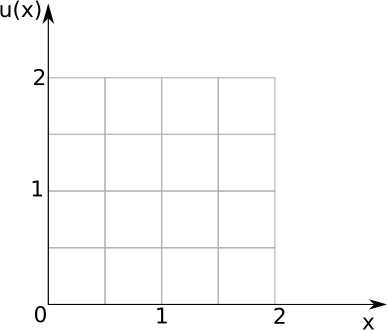
\includegraphics[width=0.6\textwidth]{figs/1d-beam-fem-empty.png}
	\end{figure}
}
\end{frame}

\note{The finite element solution is exact at the nodes, but it is not exact between the nodes. 
	This `\textit{exactness}' is a feature of finite element methods in one dimension, but it 
	does not carry over to higher dimensions.\\ 
	
	Since the exact solution is quadratic, the finite element solution would be exact if you 
	use elements which are quadratic or higher.}

\section{A case-study of a FE failure}
%-----------------------------------------------------------------
\begin{frame}
\frametitle{Sleipner A offshore platform sprang leak}
	\begin{figure}
	\centering
	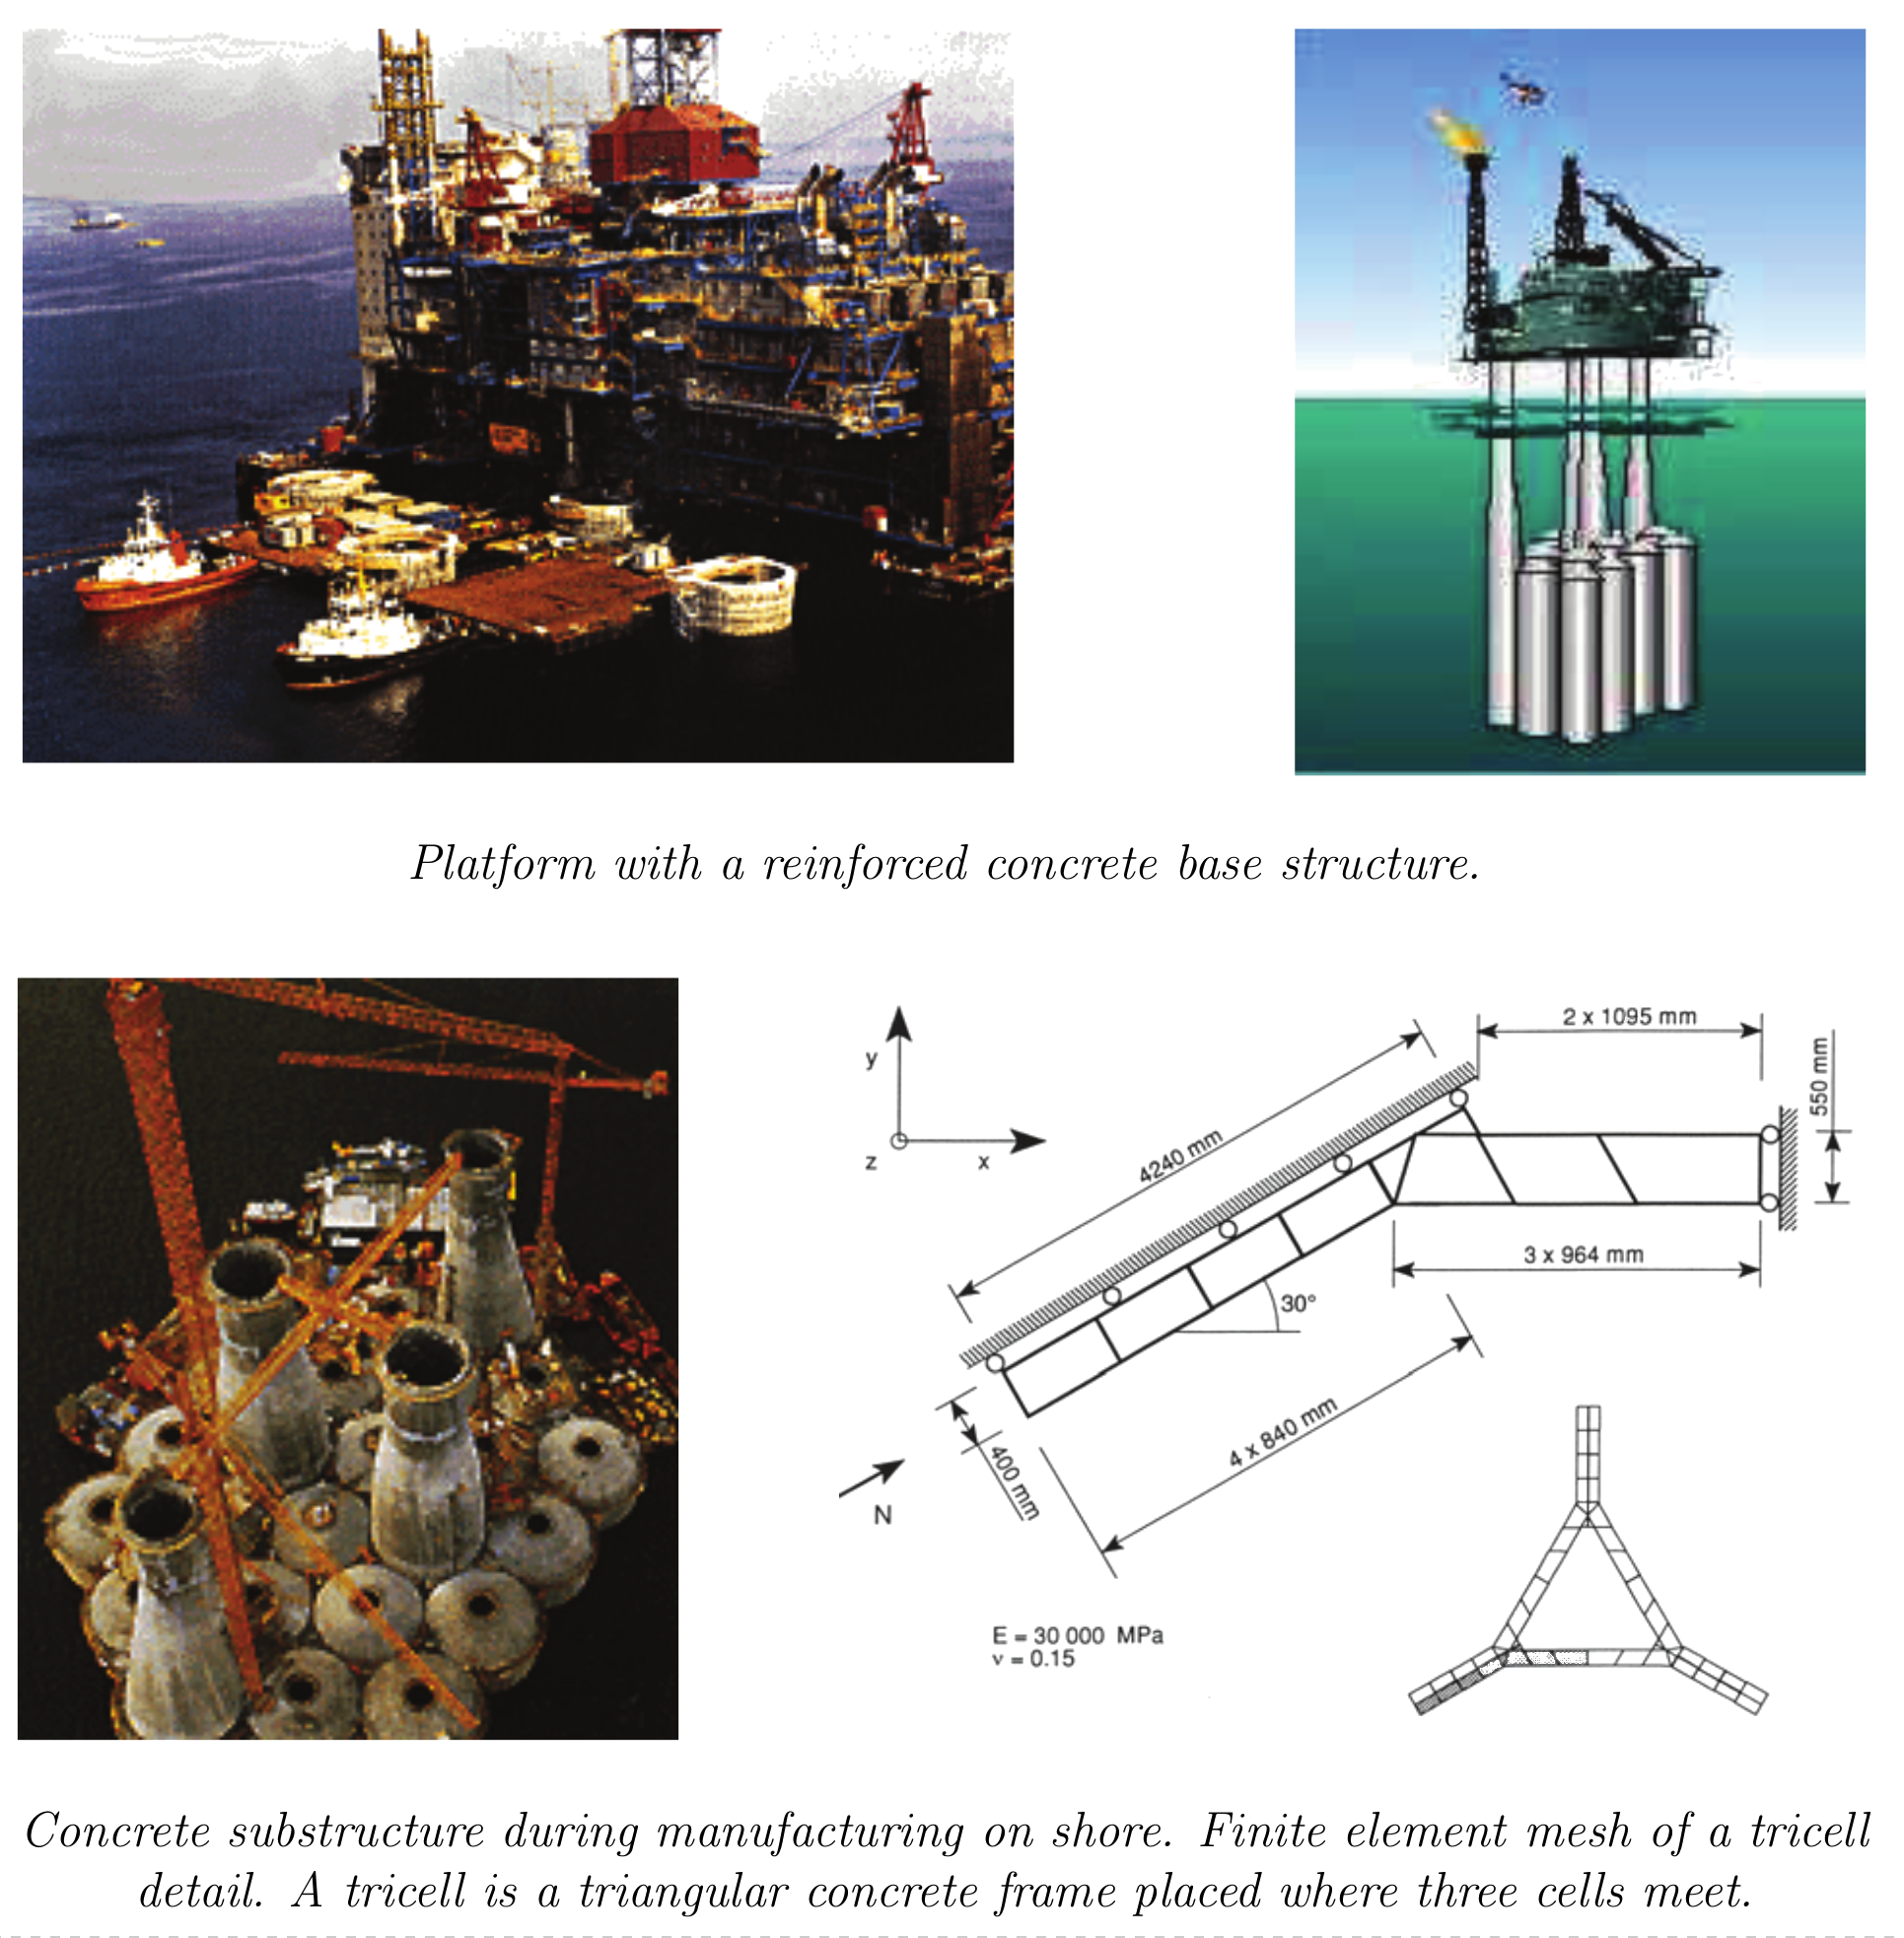
\includegraphics[width=0.6\textwidth]{figs/sleipner.png}
\end{figure}
\end{frame}

%-----------------------------------------------------------------
\begin{frame}
\frametitle{Sleipner A offshore platform sprang leak}
\begin{figure}
	\centering
	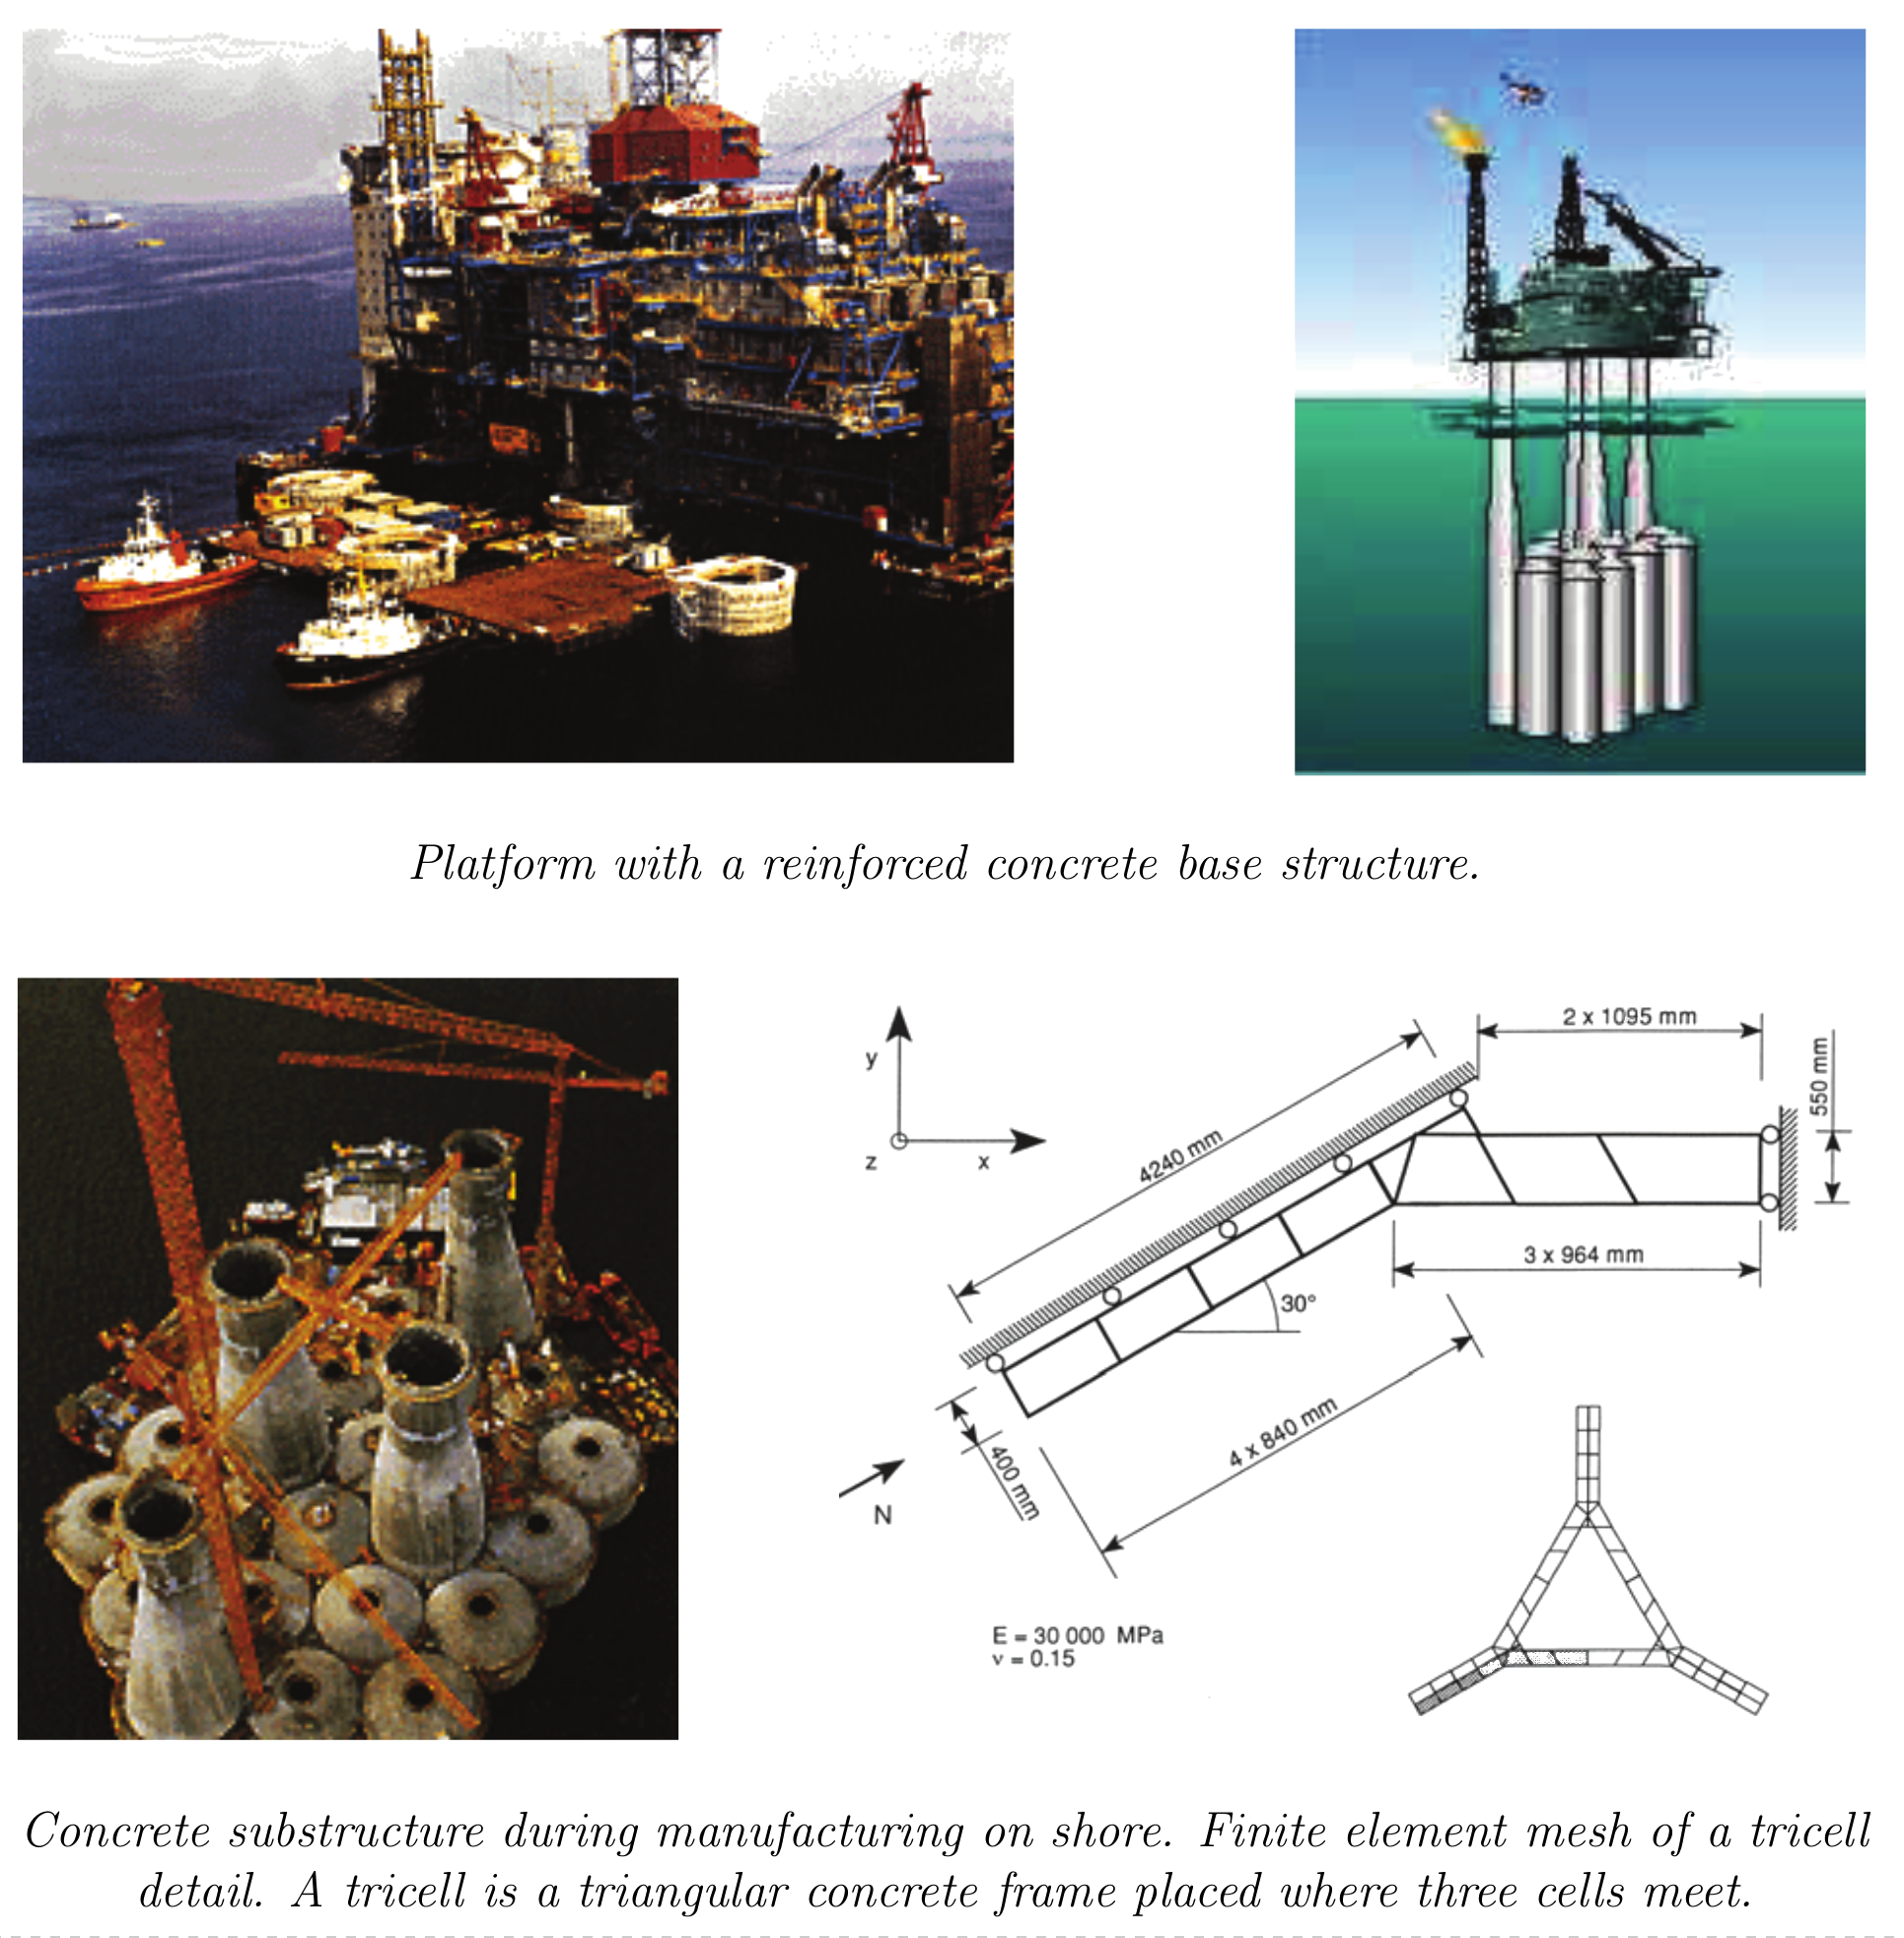
\includegraphics[width=0.5\textwidth]{figs/sleipner.png}
	\caption*{Using the FE program NASTRAN, the shear stresses in the tricells were under-estimated by 47\%. First, the chosen finite element mesh was exceedingly coarse so that the finite element shear stress was significantly too small.}
\end{figure}
\end{frame}

%-----------------------------------------------------------------
\begin{frame}
\frametitle{Sleipner A offshore platform sprang leak}
\begin{figure}
	\centering
	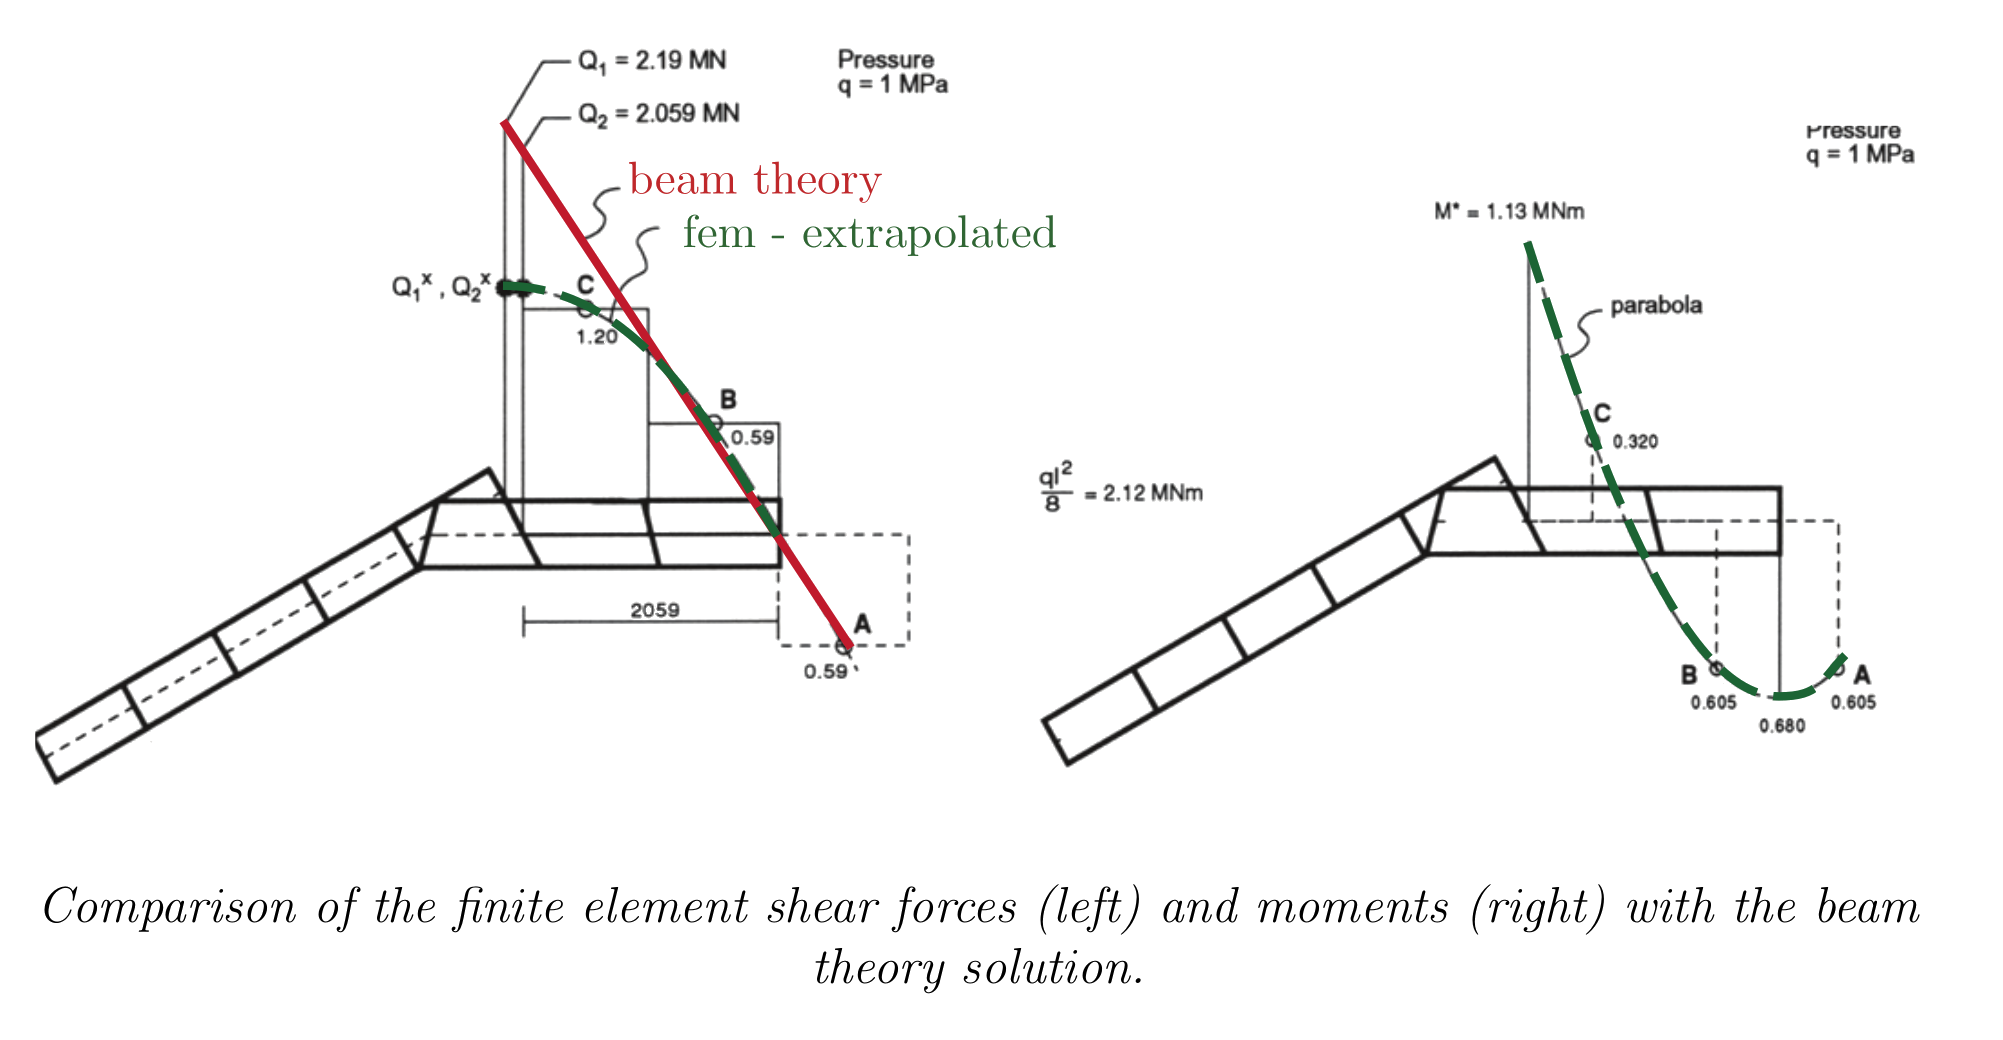
\includegraphics[width=0.9\textwidth]{figs/sleipner-shear.png}
	\caption*{Second, the shear stresses at the boundary have been quadratically extrapolated using the shear forces at points A, B and C. We know however from beam theory that the shear force distribution is linear so that the shear force at the boundary is underestimated by $\approxeq$ 40\%}
\end{figure}
\end{frame}

%-----------------------------------------------------------------
\begin{frame}
\frametitle{Sleipner A offshore platform sprang leak}
\begin{figure}
	\centering
	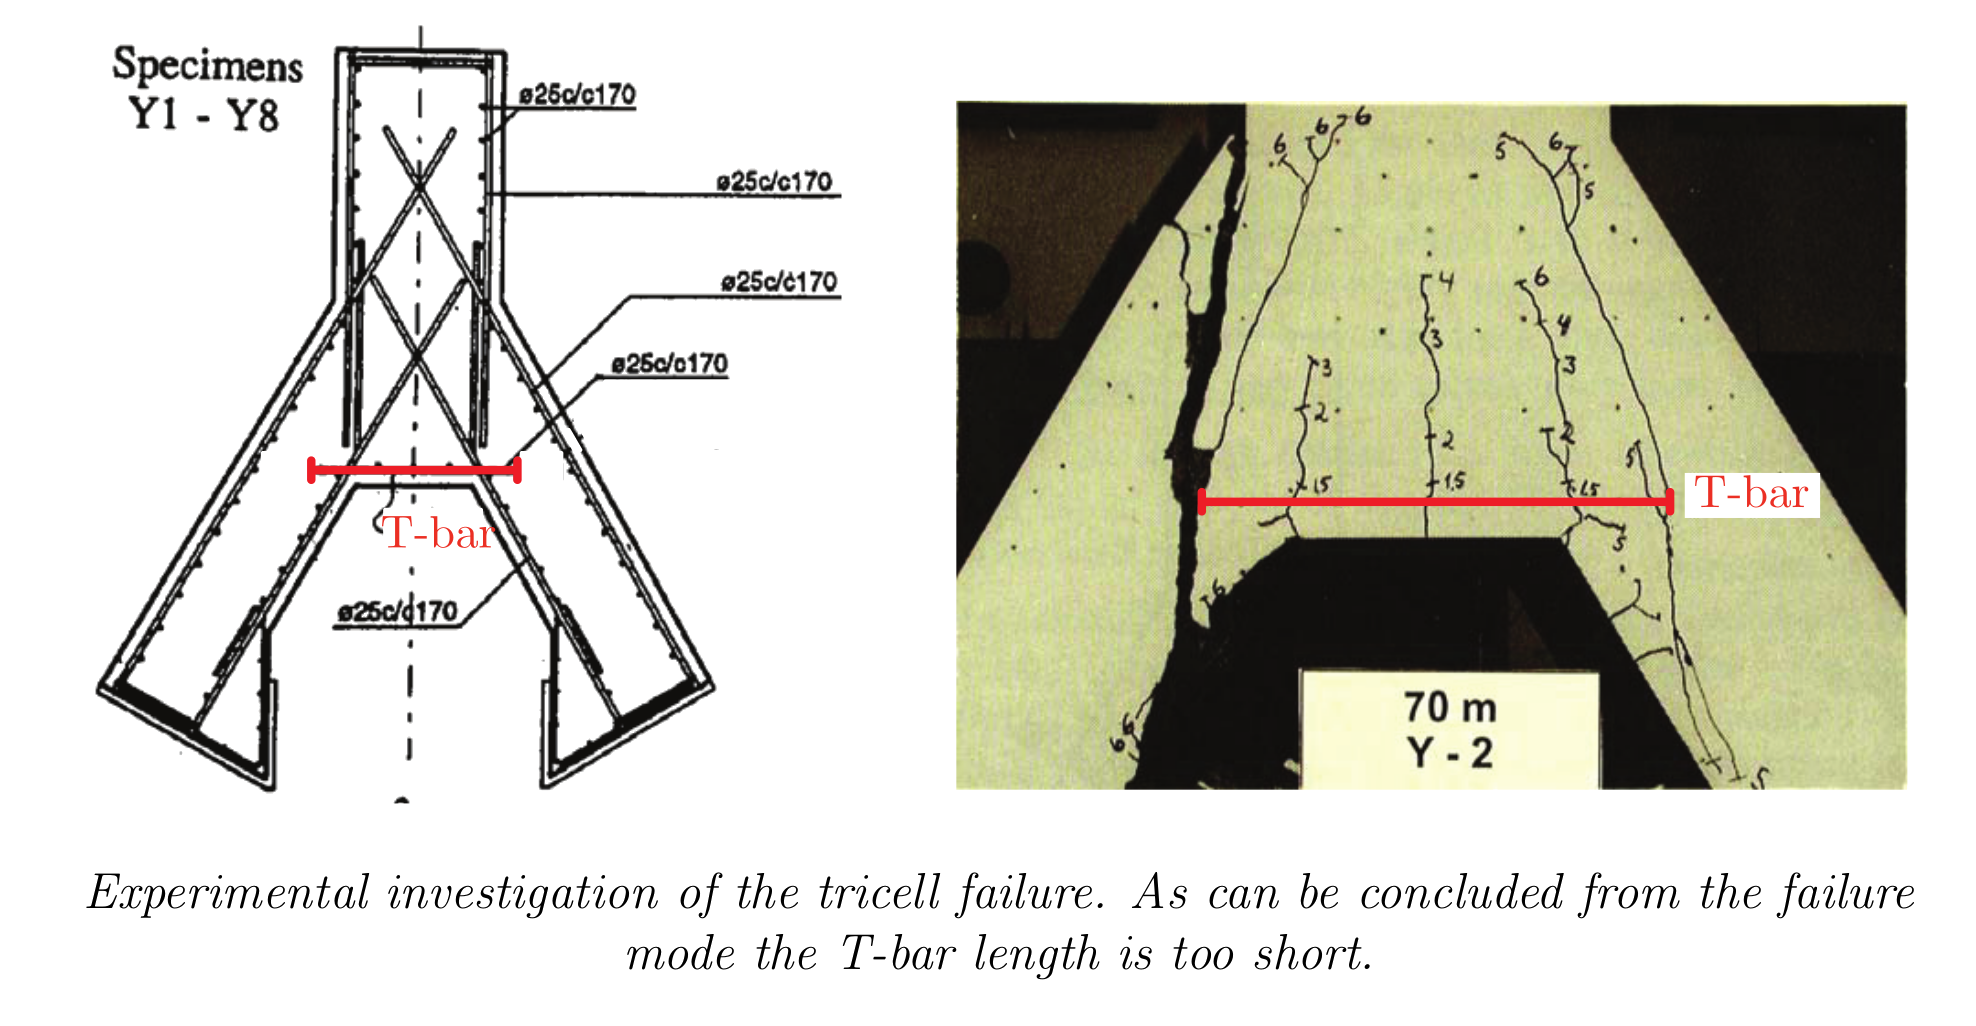
\includegraphics[width=\textwidth]{figs/sleipner-reinforcement.png}
	\caption*{To make matters worse, the necessary reinforcement was automatically 
		dimensioned based on the FE results without any checking by an engineer.}
\end{figure}
\end{frame}

\section{2D truss analysis}
%-----------------------------------------------------------------
\begin{frame}
\frametitle{2D truss analysis}
Consider the following structural system consisting of a three-noded triangle and a cable
element (i.e. two-noded one-dimensional element):

\begin{figure}
	\centering
	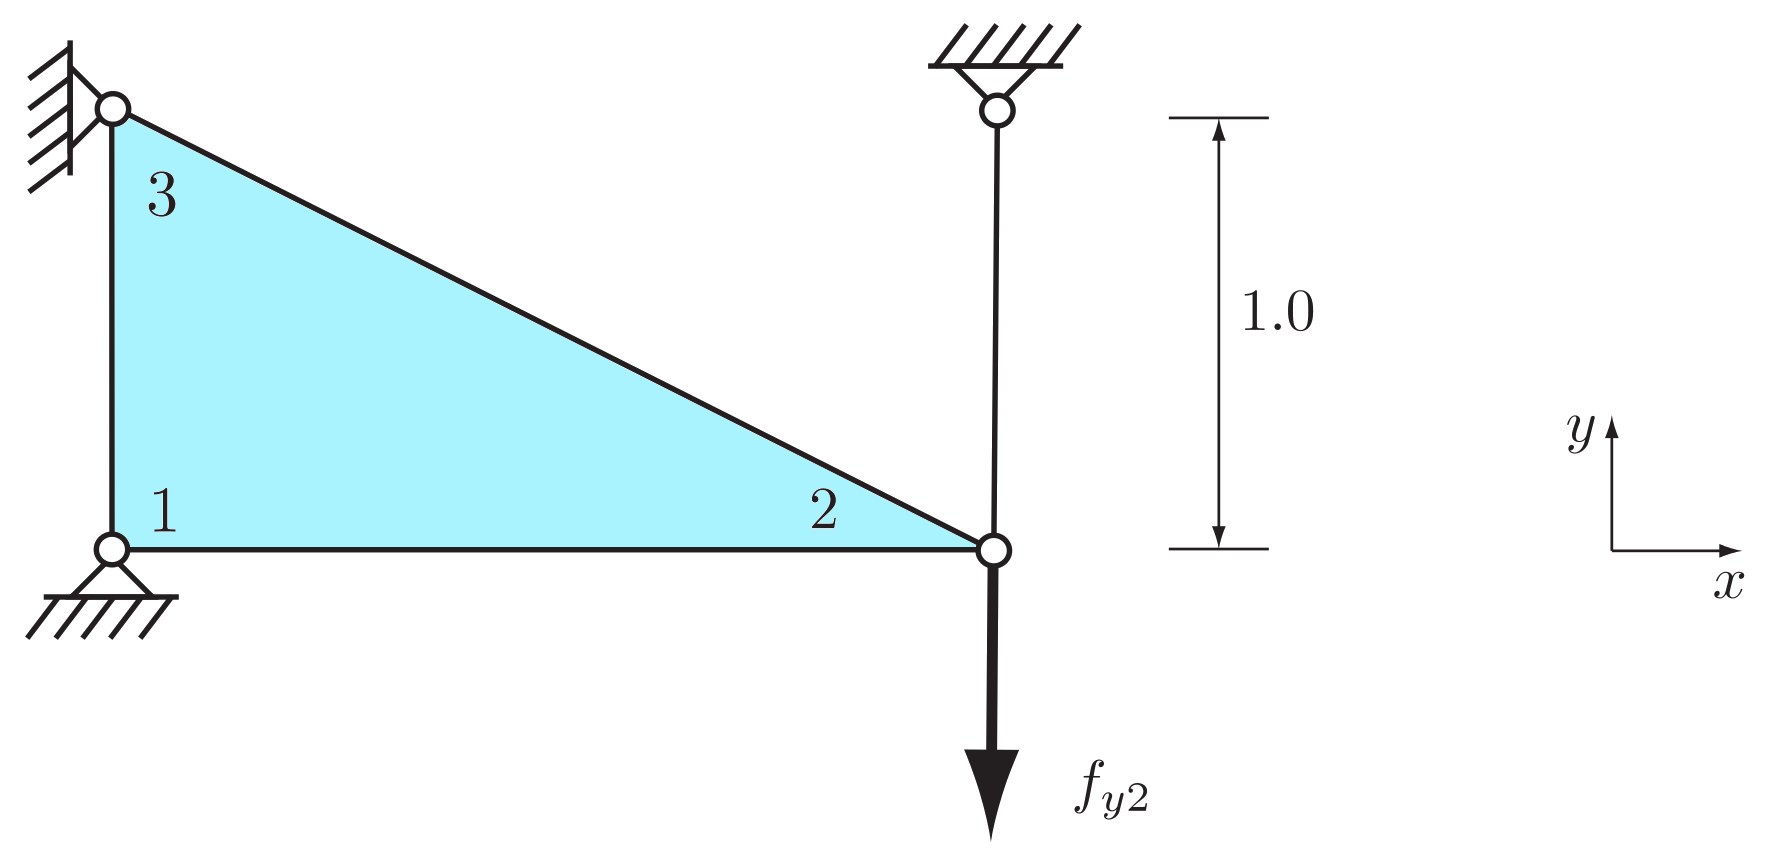
\includegraphics[width=0.85\textwidth]{figs/2d-truss.png}
\end{figure}
\end{frame}


%-----------------------------------------------------------------
\begin{frame}
\frametitle{2D truss analysis}

The triangle element is fixed at the (local) nodes 1 and 3 and its stiffness matrix for the
unconstrained degrees of freedom at node 2 is

\begin{equation*}
\mathbf{K} = 10^9 %
\begin{bmatrix}
1.97	& 0 \\ 
0 & 0.66 \\
\end{bmatrix}
%
\begin{matrix}
u_{x2}^e\\ 
u_{y2}^e \\
\end{matrix}	
\end{equation*}

For the cable, the product of the Young’s modulus and cross-sectional area is $EA = 1.0\cdot 10^9$.
Further, the system is loaded with a nodal force of $f_{y2} = -10000$.

Inserting $EA$ and the length $h = 1.0$ gives the stiffness matrix for a two-noded one-dimensional element as:
\mode<beamer>{
	\begin{equation*}
	\mathbf{K}^e = \frac{EA}{h} %
	\begin{bmatrix}
	1 & -1 \\
	-1 & 1 \\
	\end{bmatrix} = 10^9 %
	\begin{bmatrix}
	1 & -1 \\
	-1 & 1 \\
	\end{bmatrix}
	\end{equation*}
}
\mode<handout>{
	\vspace{3cm}
}
\end{frame}

%-----------------------------------------------------------------
\begin{frame}
\frametitle{2D truss analysis}
To compose the global stiffness matrix we consider the correspondence between the
element specific (local) degrees of freedom of the triangle and the cable

\begin{figure}
	\centering
	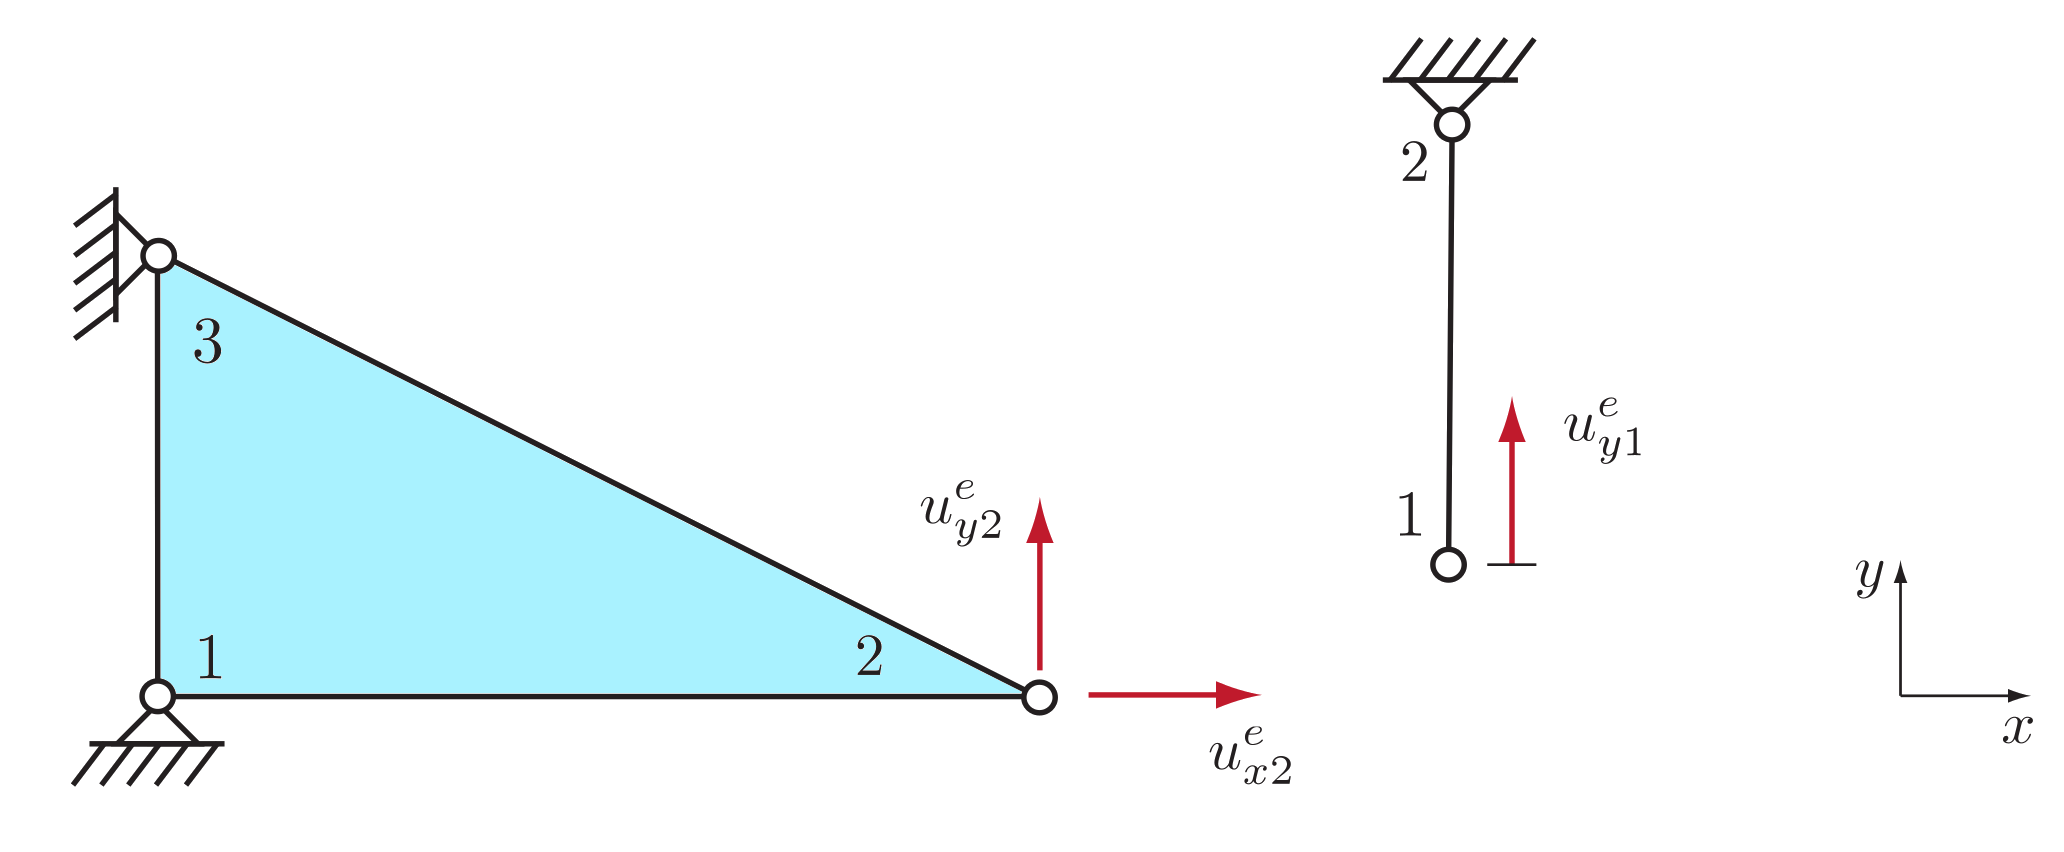
\includegraphics[width=0.65\textwidth]{figs/2d-truss-solution.png}
\end{figure}

In the global stiffness matrix, the element stiffness matrix components corresponding
to $u^e_{y2}$ of the triangle and $u^e_{y1}$ of the cable are add up:

\mode<beamer>{
	\begin{equation*}
	\mathbf{K}^e = 10^9 %
	\begin{bmatrix}
		1.97 &  0 \\
		0 & 1 + 0.66\\
	\end{bmatrix}
	\end{equation*}
}
\mode<handout>{
	\vspace{3cm}
}
\end{frame}

%-----------------------------------------------------------------
\begin{frame}
\frametitle{2D truss analysis}
Hence, the final equation system for determining the nodal displacements is:
\mode<beamer>{
	\begin{align*}
	10^9 %
	\begin{bmatrix}
	1.97 &  0 \\
	0 & 1.66\\
	\end{bmatrix} %
	\begin{bmatrix}
		u_x\\
		u_y\\
	\end{bmatrix} & = %
	\begin{bmatrix}
		0 \\
		-1000\\
	\end{bmatrix} \qquad (\mathbf{K a = f})\\
	%
	\begin{bmatrix}
		u_x\\
		u_y\\
	\end{bmatrix} & = %
	\begin{bmatrix}
		0 \\
		6.02 \times 10^{-06}\\
	\end{bmatrix}
	\end{align*}
}
\mode<handout>{
	\vspace{3cm}
}
\end{frame}
\end{document} 


